
\begin{questions}
\question{
Simple Cubic
}
\begin{solution}
Before all this we need to perform a quick calculation to know the radius of the atoms, assuming they are spherical and have a volume equal to $V_{atom}$,
\begin{equation}
  \begin{aligned}[b]
    V_{atom} &= \frac{4}{3}\pi r^3,\\
    \Rightarrow r_{atom} &= \left(\frac{3V_{atom}}{4\pi}\right)^{1/3}.
  \end{aligned}
  \label{radius}
\end{equation}


\begin{center}
  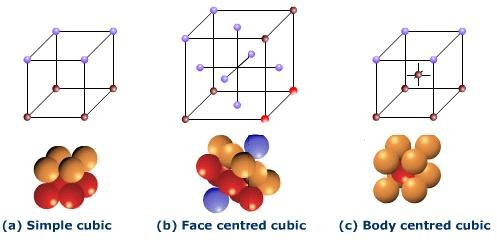
\includegraphics[width=95mm]{cells}
\end{center}

\captionof{figure}{a) SC, b) FCC and c) BCC unit cells (image taken from \textit{http://chem-guide.blogspot.de/2010/04/simple-cubic-face-centered-and-body.html}).}\label{u:cells}\vspace{0.5cm}

Now that we know this we can start with the main calculations. First the atomic packing factor for the SC unit cell. For this cell we have atoms placed at the corners of a cube. They touch along the side of the cube as we can see in fig. \ref{u:cells}. Hence the length of the size of the cube is
\begin{equation*}
  a = r + 2 = 2r,
\end{equation*}
So the volume of the unit cell is
\begin{equation}
  V_{cell} = a^3 = 8r^3 =8\frac{3V_{atom}}{4\pi} =\frac{6V_{atom}}{\pi},
\end{equation}
There is just 1 atom inside the unit cell, so the atomic packing factor is going to be
\begin{equation}
  APF_{SC} = \frac{NV_{atom}}{V_{cell}} = \frac{(1)V_{atom}}{\frac{6V_{atom}}{\pi}} = \hlgreen{\frac{\pi}{6}.}
\end{equation}
\end{solution}
\question{FCC}
\begin{solution}
  Now for the FCC we can see that now we have atoms at the corners and in the center of each face, so now the atoms are touching along the diagonal of the faces of the cube. So the diagonal size must be
  \begin{equation}
    c = r + 2r + r = 4r,
  \end{equation}
  but we are not interested in the diagonal, we want to know the size of the sides. We can obtain such sides with basic trigonometry, if $a$ is the side length then
  \begin{equation}
    \begin{aligned}[b]
      c^2 &= (4r)^2 = 16r^2, \\
      c^2 &= a^2 + a^2 = 2a^2,\\
      \Rightarrow 8r^2 &= a^2\\
      \Rightarrow a &= \sqrt{8}r.
    \end{aligned}
  \end{equation}
  Therefore the volume of the unit cell is
  \begin{equation}
    V_{cell} = (\sqrt{8}r)^3 = 8\sqrt{8}r^3 = 16\sqrt{2}r^3 = 16\sqrt{2}\frac{3V_{atom}}{4\pi} = \frac{12\sqrt{2}V_{atom}}{\pi} .
  \end{equation}
  The FCC cell has 4 atoms, $8*(1/8) + 6*(1/2)$, the $1/8$ comes from the atoms on the corner that are in 8 cells simultaneously and the $1/2$ comes from the atoms in the faces that are shared by two cells each. So the packing factor is
  \begin{equation}
    APF_{FCC} = \frac{4*V_{atom}}{V_{cell}} = \frac{4*V_{atom}}{\frac{12\sqrt{2}V_{atom}}{\pi}} =  \hlgreen{\frac{\pi}{3\sqrt{2}}.}
  \end{equation}
\end{solution}

\question{BCC}
\begin{solution}
  Now it is time to do the same calculations for the BCC unit cell. In such cell we have atoms on every corner of the cube and an extra one placed at the center. So now the atoms touch each other alongside the diagonal. As a result, the diagonals of the cell have a length of
  \begin{equation*}
    c = r + 2r + r = 4r.
  \end{equation*}
  By basic trigonometry we know that the size of the diagonal of a cube is $c = \sqrt{3} a$, where $a$ is the size of each side. So the length of the diagonal in terms of the atomic radius is
  \begin{equation}
    \begin{aligned}
      \sqrt{3} a &= 4 r,\\
      \Rightarrow a &= \frac{4}{\sqrt{3}}r = \frac{4}{\sqrt{3}}\left(\frac{3V_{atom}}{4\pi}\right)^{1/3}.
    \end{aligned}
  \end{equation}
  As a consequence, the volume of the cell is
  \begin{equation}
    V_{cell} = a^3 = \frac{64}{3\sqrt{3}}\left(\frac{3V_{atom}}{4\pi}\right) = \frac{16V_{atom}}{\sqrt{3}\pi}.
  \end{equation}
  The number of atoms in a BCC cell is 2, ($8*1/8 + 1$), one in the center and 8 on the corners contributing $1/8$ each, knowing this the atomic packing factor is
  \begin{equation}
    APF_{BCC} = \frac{2*V_{atom}}{V_{cell}} = \frac{2*V_{atom}}{\frac{16V_{atom}}{\sqrt{3}\pi}} = \hlgreen{\frac{\sqrt{3}\pi}{8}.}
  \end{equation}
\end{solution}

\question{HCP}
\begin{solution}
The only remaining structure to calculate here is the HCP unit cell. In fig. \ref{hcp} we can see the scheme we will use to perform our calculations.
  \begin{center}
    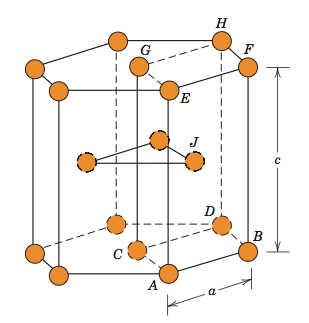
\includegraphics[width=55mm]{hpc}
  \end{center}

  \captionof{figure}{HPC structure, taken from \textit{https://www.e-education.psu.edu/matse81/node/2134}.}\label{hcp}\vspace{0.5cm}

Let's consider the tetrahedron formed by the vertexes $ABCJ$. It's is easy, with our now acquired experience, to see that atoms are touching each other alongside $AB$, and also along $BJ$, both these sides have the same length $a = 2r$. So far we are not in troubles, so let's calculate the height of the tetrahedron $c/2$. We know that the triangle $ABC$ is equilateral, as $ABJ$, $BCJ$ and $CAJ$, therefore we have a tetrahedron with equilateral triangles as faces, so $J$ must lie right above the centroid of the triangle

\begin{center}
  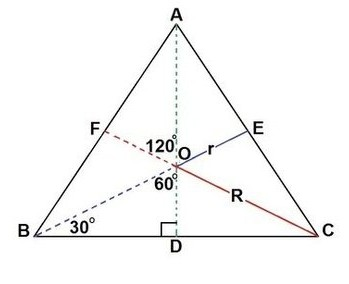
\includegraphics[width=55mm]{centroid}
\end{center}

\captionof{figure}{Centroid of an equilateral triangle, taken from \textit{https://www.quora.com/What-is-the-centroid-of-equilateral-triangle}.}\label{centroid}\vspace{0.5cm}

In fig. \ref{centroid} we want to know the length of $BO$, we know that $BD = a/2$, if we use the definition of cosine then we will find
\begin{equation}
  \begin{aligned}[b]
    \cos(30^\circ) &= \frac{\sqrt{3}}{2} = \frac{BD}{BO}, \\
    \Rightarrow BO &= \frac{2BD}{\sqrt{3}} = \frac{a}{\sqrt{3}}
  \end{aligned}
  \label{bo}
\end{equation}
Now using Pythagoras theorem we find $OJ$ (remember that $OJ = c/2$)
\begin{equation}
  \begin{aligned}[b]
    BJ^2 &= BO^2 + OJ^2,\\
    a^2 &= \frac{a^2}{3} + OJ^2,\\
    OJ &= \frac{\sqrt{2}a}{\sqrt{3}},
  \end{aligned}
\end{equation}
then
\begin{equation}
  c = 2OJ = \frac{2\sqrt{2}a}{\sqrt{3}}.
\end{equation}

We almost finish, we just need to know the apothem size ($CF$), this can be easily calculated with Pythagoras theorem and eq. \ref{bo}
\begin{equation}
  \begin{aligned}[b]
    CF^2 &= a^2 - \frac{a^2}{4} = \frac{3a^2}{4},\\
    \Rightarrow CF &= \frac{\sqrt{3}a}{2}.
  \end{aligned}
\end{equation}
The area of the base hexagon is then
\begin{equation}
  Area_{hex} = \frac{6a*CF}{2} =  \frac{3\sqrt{3}a^2}{2},
\end{equation}
hence the volume of the unit cell is
\begin{equation}
  \begin{aligned}
    V_{cell} &= c*Area_{hex} = \frac{2\sqrt{2}a}{\sqrt{3}}\frac{3\sqrt{3}a^2}{2} \\  &= 3\sqrt{2}a^3 = 3\sqrt{2}(2r)^3 = 24\sqrt{2}r^3 = \\
     &=24\sqrt{2}\frac{3V_{atom}}{4\pi} = \frac{18\sqrt{2}V_{atom}}{\pi}.
  \end{aligned}
\end{equation}
And finally we can calculate the atomic packing factor. In the hcp cell there are 6 atoms ($6*1/4 + 3$), hence we have
\begin{equation}
  APF_{HCP} = \frac{6*V_{atom}}{V_{cell}} = \frac{6*V_{atom}}{\frac{18\sqrt{2}V_{atom}}{\pi}} = \hlgreen{\frac{\pi}{3\sqrt{2}}.}
\end{equation}
\end{solution}

\question{Crystal structure of iron}
\begin{solution}
  This one might be tricky. Let's first define the density in the unit cell.
  \begin{equation}
    \rho = \frac{N M_{atom}}{V}.
  \end{equation}
  Assuming we have a cubic cell, we can use $V=a^3$. Hence, from the density, mass, and volume, we can know how many atoms are there inside the unit cell.
  \begin{equation}
    N = \frac{\rho V}{M_{atom}}.
  \end{equation}
  If we plug the numbers in the computer (using the appropiate units), we will find that $N\approx2.0022590256465516$, which is very close to 2. And two is the number of atoms inside a BCC cell. Therefore \textbf{the crystal structure of the iron is BCC.}
\end{solution}
\end{questions}

%
% \begin{center}
%   \includegraphics[width=55mm]{}
% \end{center}
%
% \captionof{figure}{}\label{new}\vspace{0.5cm}
